Based on the analysis, as one of the most advanced documentation generators is Swagger UI, it will be my main inspiration.
Also, the Swagger UI is a well-known tool in the software development community, and many companies and projects use it.
The Swagger UI works so the website is static by default, and the endpoints, types, and more are defined in a definition file.
This file is an OpenAPI YAML or JSON file, which is then parsed and displayed on the website~\cite{swagger-ui-definition-file}.
This is a good approach, as it separates the data from the view.
This allows the data to be easily changed, and the website will regenerate dynamically in the browser.
The deployment of the website is also more accessible, as it is just a static website, which can be hosted on any web server, and updating the definitions can be part of different deployment processes.

First, I will analyze if I could use Swagger UI directly or if I need to create my own website.


\section{Swagger UI for gRPC}
The first idea is to use Swagger UI and generate the OpenAPI definition file from the gRPC proto files.
This approach would benefit from reusing a known tool with all its features.
The issue is that OpenAPI Specification is made for HTTP APIs, which gRPC APIs, although using HTTP/2, are not~\cite{openapi-specification}.
This means the OpenAPI Specification does not support gRPC specifics, like the streaming or mapping service methods to HTTP endpoints.
Implementation of such would require compromises on the translation layer between the two.
As described in the analysis, the gRPC-Gateway is an example of this translation, but it is not a perfect solution, and it has its limitations, which I want to avoid.

Another option is using the Swagger UI plugin system~\cite{swagger-ui-plugins}.
This would allow me to use the swagger-ui package as a dependency and build all the gRPC specifics on top of it, including reading different specifications than OpenAPI\@.
The positive side of this approach is that I would be able to use the Swagger UI design.
On the other hand, I would need to reimplement almost every single part in order to be able to work with gRPC specifics and, in the future, maintain compatibility with possible Swagger UI updates.
This would leave me only with a page skeleton.
That is a toolbar and a background color.
I do not see that as a significant advantage over creating my own website.

In the end, I have decided to create my own website, which will be inspired by the Swagger UI design, but it will be adjusted to the gRPC specifics.


\section{gRPC-Web Limitations}
% gRPC-Web limitations and how they affect the design
% Possibility of full gRPC server implementation in the future, but also may not be necessary if gRPC-Web supports it
% grpc-web-text and grpc-application content types
Previously, I mentioned the limitations of the gRPC-Web.
The most important influence will be based on the lack of support for client streaming and bidirectional streaming, even though its implementation is on the roadmap.
This means that the website will not be able to execute these method types, and the execution will be limited to unary and server streaming methods only.
However, it does not affect the design of the website.
It can still show all relevant documentation and have the implementation ready when gRPC-Web developers add support.

For the possibility of gRPC-Web support for client streaming and bidirectional streaming not being added in the following years, I will prepare an interface to use a custom gRPC server proxy.
If an implementation of that interface is provided, the website will be able to use it, and the user will be able to use all gRPC methods, including client streaming and bidirectional streaming.
This solution will not be part of my thesis, but I will prepare the website so it can be added (or removed altogether) in the future.


The server streaming also has a limitation in gRPC-Web, which is that it works only in \textit{application/grpc-web-text} format~\cite{grpc-web}.
This means that the payload is base64 encoded, and it is not possible to use the \textit{application/grpc-web+proto} content type, which uses payload in binary format.
Only unary calls support both \textit{an application/grpc-web+proto} and \textit{application/grpc-web-text} content types.
Therefore, unary requests will feature a selection of content types, which users will be able to change.


\section{gRPC Reflection Possibility}
% Discuss the options and possibilities
Before I start designing the website architecture, I need to decide how the gRPC reflection as a data source could be used compared to the proto files.
Any tool using gRPC reflection has to support the connection using gRPC itself.
Therefore, it is not possible to use it directly in the browser.
A server-side tool or client will need to be used to connect to the gRPC server and get the reflection data.
The grpcurl tool mentioned in the analysis allows not only creating the client but also exporting a \enquote{protoset} file.
This is a file containing the reflection metadata in its own format.
This file can be used instead of a direct gRPC server as a reflection source.
But it can also be read with tools other than grpcurl.
For example, the gRPC UI tool elevates this in its own implementation~\cite{grpc-grpcui}.
This will allow for the documentation website to either use the protoset file directly or convert the protoset file to a different common format, which the website will then use.

% Issue with comments in reflection, reflection feasibility
The limitation of the gRPC reflection is that it does not provide comments from the proto files.
This means the website will not be able to show the comments, which are part of the proto files, if the reflection is used.
This is a significant limitation, as the comments are part of the documentation, and they are important for the user to understand the methods and types.
The good thing is that it is being tracked on GitHub (\url{https://github.com/grpc/grpc/issues/22680}) by the gRPC developers, and when it is implemented, the documentation website will be able to use it.
For now, if documentation comments are required, the proto files will have to be used as the data source.


\section{Architecture}
The architecture of the website will be based on the Swagger UI, but it will be adjusted to the gRPC specifics.
The website will be static, and it will take a gRPC definition file to show all gRPC-related parts.
The gRPC definition file from the proto files or gRPC reflection and its format will be most probably either JSON or YAML\@.
These formats are common in software development, and they are also used by the Swagger UI, from which I take inspiration.

I have created a diagram of the website architecture, which is shown in the figure~\ref{fig:grpcflair-architecture}.
There are two places where the generation of the common format starts.
The first one is from the .proto file.
The second one is from the gRPC reflection.
Both methods will generate the same format that the website will use.
The website will be static and generated using the common format on the fly using client-side programming languages like JavaScript.
The user of the website will be able to see all the methods, types, and enums, which are defined in the gRPC definition file.
They will also be able to call the methods and see the responses on the website.
When they invoke the request, the website will select the correct backend (gRPC-Web or other implementation), and it will be the server.
The server then returns the response, which is then displayed on the website (the responses can be shown gradually as, for example, the server streams responses).

% The overall process description - state diagram - (with the help of the diagram I have)
% Swagger UI JSON inspiration

\begin{figure}[hbt!]
    \centering
    \captionsetup{justification=centering}
    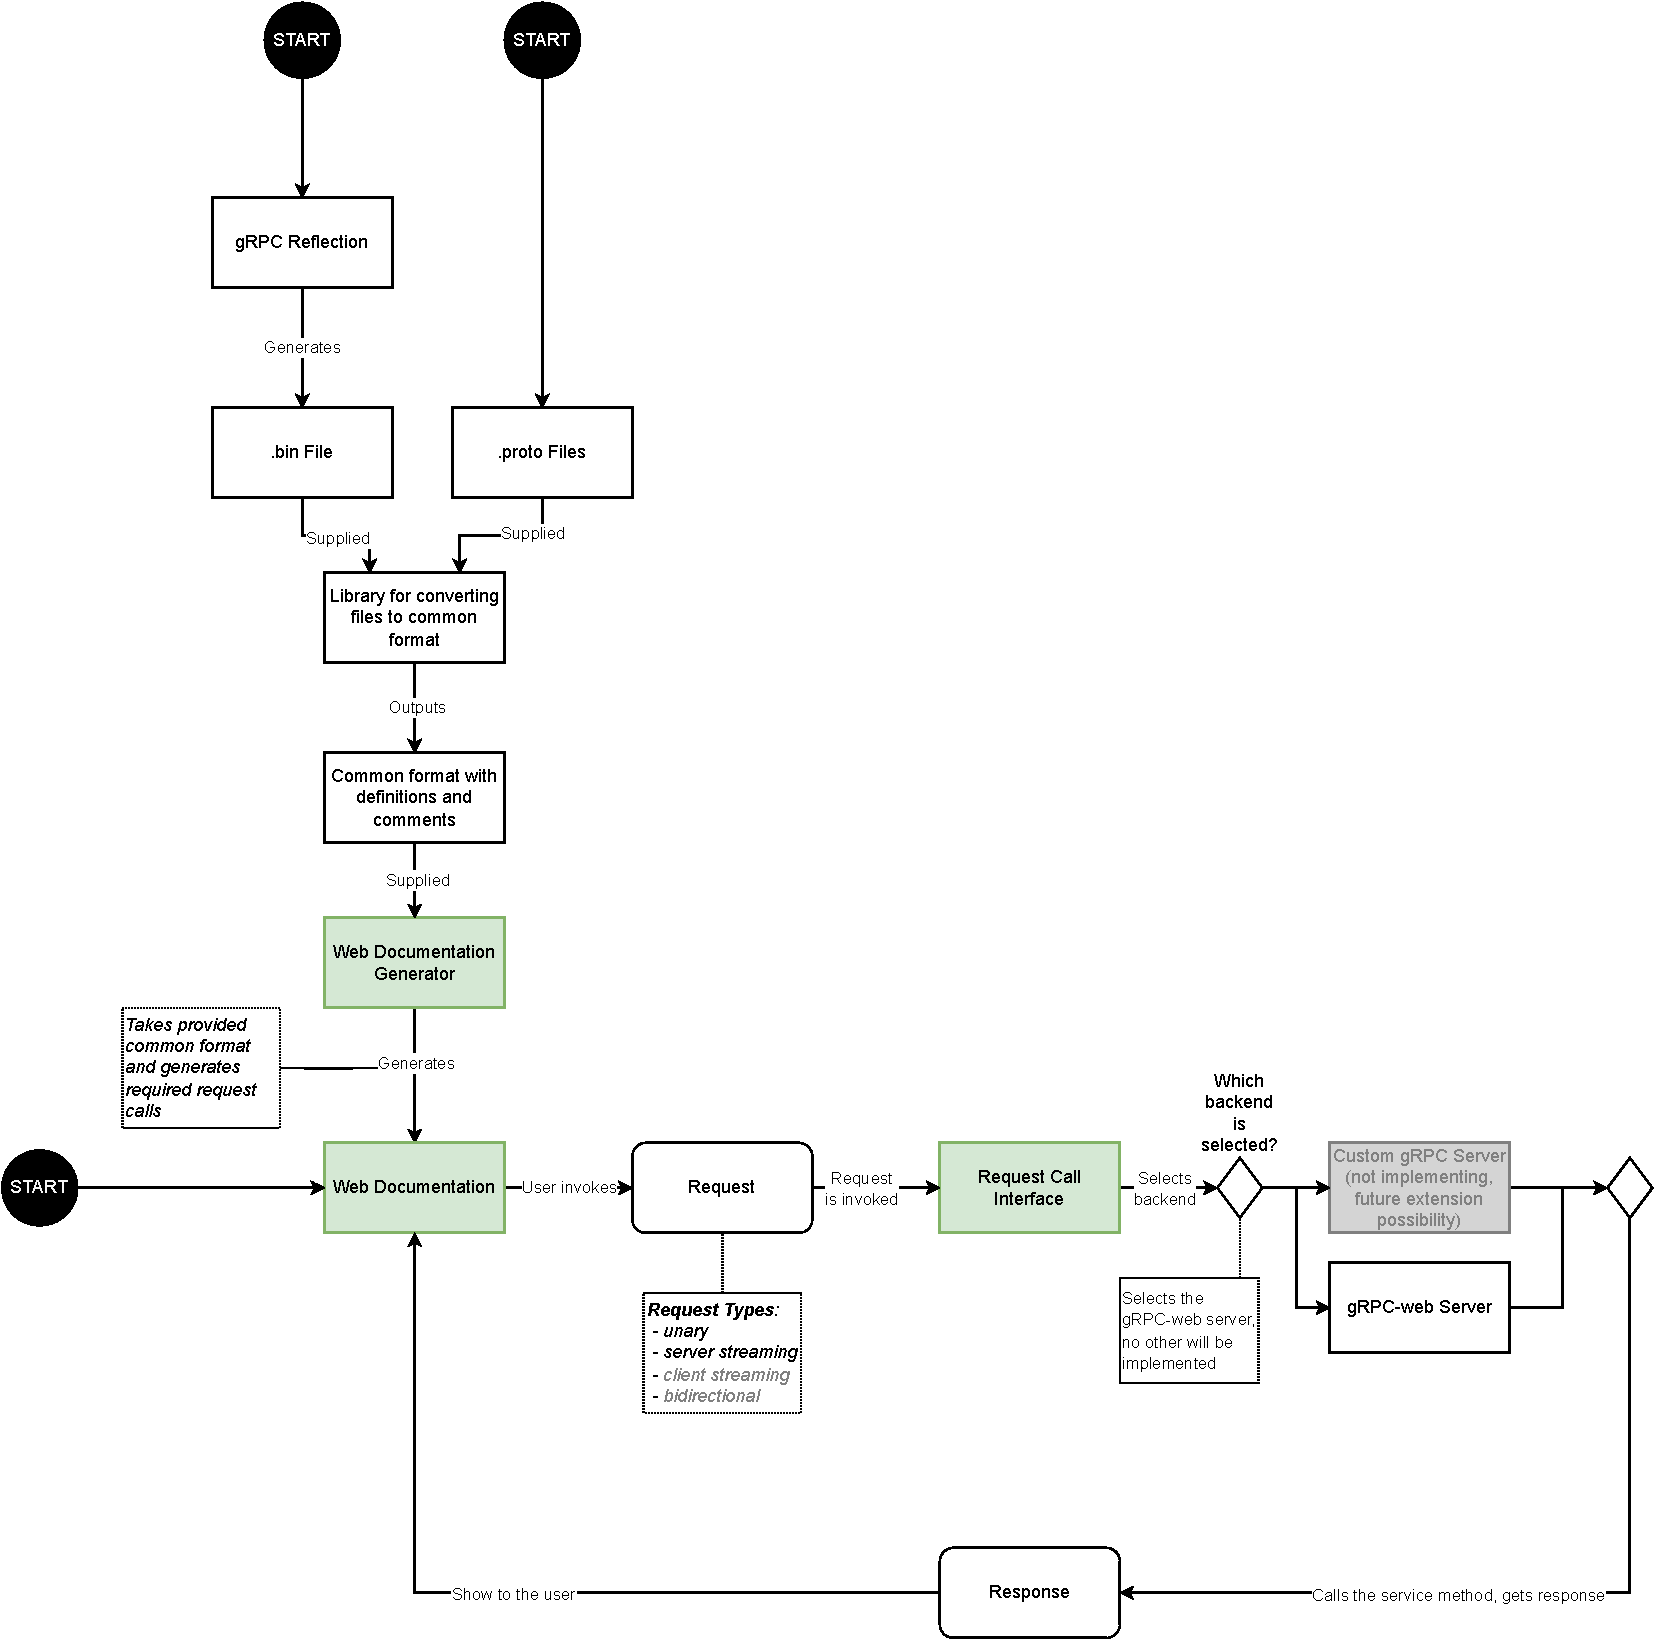
\includegraphics[width=1.0\textwidth]{images/design/grpcdoc-architecture}
    \caption{Architecture}
    \label{fig:grpcflair-architecture}
\end{figure}

This architecture should allow static website hosting, with the possibility of generating the website on the fly based on the common format definition.
The deployment of that website could be then split into deploying the website itself and deploying the common format definition, which may allow more possibilities for gRPC API developers or maintainers.
It will be also able to execute queries and, more importantly, show server streaming responses right at the moment they are received from the server.
The website will be able to work with both proto files and gRPC reflection, and it will be ready for future gRPC-Web support for client streaming and bidirectional streaming.


\section{Common Format}
As previously mentioned, the website will use a common format for the gRPC definitions, from which the website will be generated on the fly.
In this section, I will discuss the possibilities of already existing common formats, and I will choose the most suitable one for the website.
I will not consider the OpenAPI standard anymore, as I have discussed previously in the Swagger UI possibility.

\subsection{grpc-protoc-gen-doc}
The grpc-protoc-gen-doc\footnote{\url{https://github.com/pseudomuto/protoc-gen-doc}} allows JSON output generation, including comments.
This is great for documentation, but it does not allow the generation of the necessary gRPC metadata used for constructing gRPC requests.
That means the website would not allow gRPC methods to be executed just from this file, and additional metadata would be needed.

\subsection{gnostic}
The gnostic\footnote{\url{https://github.com/google/gnostic}} is a compiler for APIs described by the OpenAPI Specification.
It generates JSON and YAML OpenAPI descriptors to (and from) Protocol Buffer representations.
It uses gRPC options to specify HTTP paths and other information.
\cite{gnostic}

This is a good option, as it is able to generate the OpenAPI Specification from the proto files.
The issue is that the binary format of the proto files is defined by gnostic, so all generations have to be done from YAML or JSON, not from the proto files at all.
This makes this library not suitable for use as a common format, as it would require the proto files to be converted to YAML or JSON first.
Or implementing a script for converting proto files to the gnostic binary format, which is still missing all the implementation needed for the website itself.

%\subsection{proto3-json-serializer}

\subsection{protobufjs}
% Protobufjs, protobufjs-cli
The protobufjs\footnote{\url{https://github.com/protobufjs/protobuf.js}} library is a JavaScript implementation with TypeScript support of the Protocol Buffers serialization with over fourteen million downloads per week.
It is able to parse the proto files and query the data from them.
The data can then be used to serialize and deserialize the messages in binary format when used in gRPC calls.
It does not execute the gRPC calls directly, but this functionality can be implemented using other libraries.
\cite{protobufjs}

This library allows for listing all services, methods, types, enums, and all other related parts of proto files, such as fields, options, and, most importantly, also comments.
It is able to parse the proto files and generate a JSON output, which can be then used instead of the proto files directly.
This is a possible candidate for the common format, as it is able to generate the necessary data for the website, and it is also able to generate the binary format for the gRPC calls.

There is also a protobufjs/ext/descriptor\footnote{\url{https://github.com/protobufjs/protobuf.js/blob/master/ext/descriptor/README.md}} extension, which is able to parse and decode the descriptor.proto files used in the binary format of gRPC reflection.
This means that the protobufjs library is able to work with both proto files and gRPC reflection.
Using this extension, I can generate the common JSON format, and the website will be able to work with the reflection too.

\subsection{Summary}
% Why protobufjs is the best option
% Why not use my own parsing

Based on the options I have found, the protobufjs library looks like the best option for the common format.
It is able to generate the JSON output, which can be used as a common format for the proto files and the gRPC reflection.
It also allows the creation of the binary message format necessary for the gRPC calls.
It is also able to parse the comments from the proto files, which is important for documentation purposes.

I could also create my own parser, which would parse the proto files and generate the JSON output.
But this would require a lot of work, and it would not be as good as the protobufjs library, which is already broadly used.
Therefore, I have decided to use the protobufjs library for the common format.


\section{Website Design}
Based on the architecture, the website generator will contain three parts:
\begin{itemize}
    \item proto files generator,
    \item gRPC reflection generator,
    \item static website.
\end{itemize}

The proto files generator will generate the JSON output from the proto files.
The gRPC reflection generator will generate the JSON output from the gRPC reflection.
The static website will take the JSON output and generate the website on the fly in the browser.

The website design will be inspired by the Swagger UI design, but it will be adjusted to the gRPC specifics.
This should allow the developers to get familiar with the website quickly, as they may already know the Swagger UI design.

I will describe each part in more detail in the following sections, and I will also show the wireframes of the website.

\subsection{Proto Files Generator}
The proto files generator will be a command line script that takes the proto files as input and generates the JSON output.
It should also allow the user to use a folder of proto files.
The protobufjs library will define the JSON output and should contain all the necessary data for the website, such as services, methods, types, enums, and comments.

\subsection{gRPC Reflection Generator}
The gRPC reflection generator will be a command line script that takes the gRPC reflection definition file as input and generates the JSON output.
The input bin file will be the protoset file generated by the grpcurl tool.
The protobufjs library will define the JSON output and should contain all the necessary data for the website, such as services, methods, types, enums, and comments.

\subsection{Website Wireframe}
The main website wireframe is in the figure~\ref{fig:wireframe-main-layout}.
It starts with a toolbar at the top, which contains the name of the website in the format of a logo and a definition file link with a preview button.
The definition file link will allow the user to upload the definition file, and the preview button will generate the website on the fly.
This link can be either a local file or a remote path.

Next, there is a part with a brief explanation of what this website is and what it allows.
This part may be used in the future for general gRPC API information of the particular definition file.

Then, there are settings fields and options that apply to the whole website.
The first one is a method selection.
This is a dropdown list that allows users to choose which backend implementation they want to use.
Right now, only gRPC-Web is supported, but in the future, there may be more options, such as custom gRPC server proxy or anything else.
Next is a gRPC server URL\@.
This is a text field where the user can enter the URL of the gRPC server, which is later used as the backend URL for gRPC calls.
For the gRPC-Web implementation, this URL will be the URL of the gRPC-Web proxy, such as Envoy.
The last setting is metadata.
The button will open a modal with a table where the user can enter the metadata key-value pairs.
There will be an authorization field that will allow the user to enter the authorization token, which will be used in the gRPC calls.
This field will only define an extra metadata pair with a predefined key and value prefix.

The main part of the website consists of three sections: services, types, and enums.
Each service name contains a full package path, documentation comment, and options, like \textit{java\_package}.
Services are expandable, and when expanded, they show the methods.
Each method contains the type (unary, client streaming, server streaming, or bidirectional streaming), name, and part of the documentation comment.
Methods are expandable as well, and when expanded, they show more information, which I will describe in the following section.

The message types and enums sections are similar to the services section.
Each message type or enum contains the full package path and documentation comment and can be expanded to show more information.
Enums are prefixed with the \textit{[Enum]} to distinguish them from message types, but otherwise, they share the same design.


\begin{figure}[hbt!]
    \centering
    \captionsetup{justification=centering}
    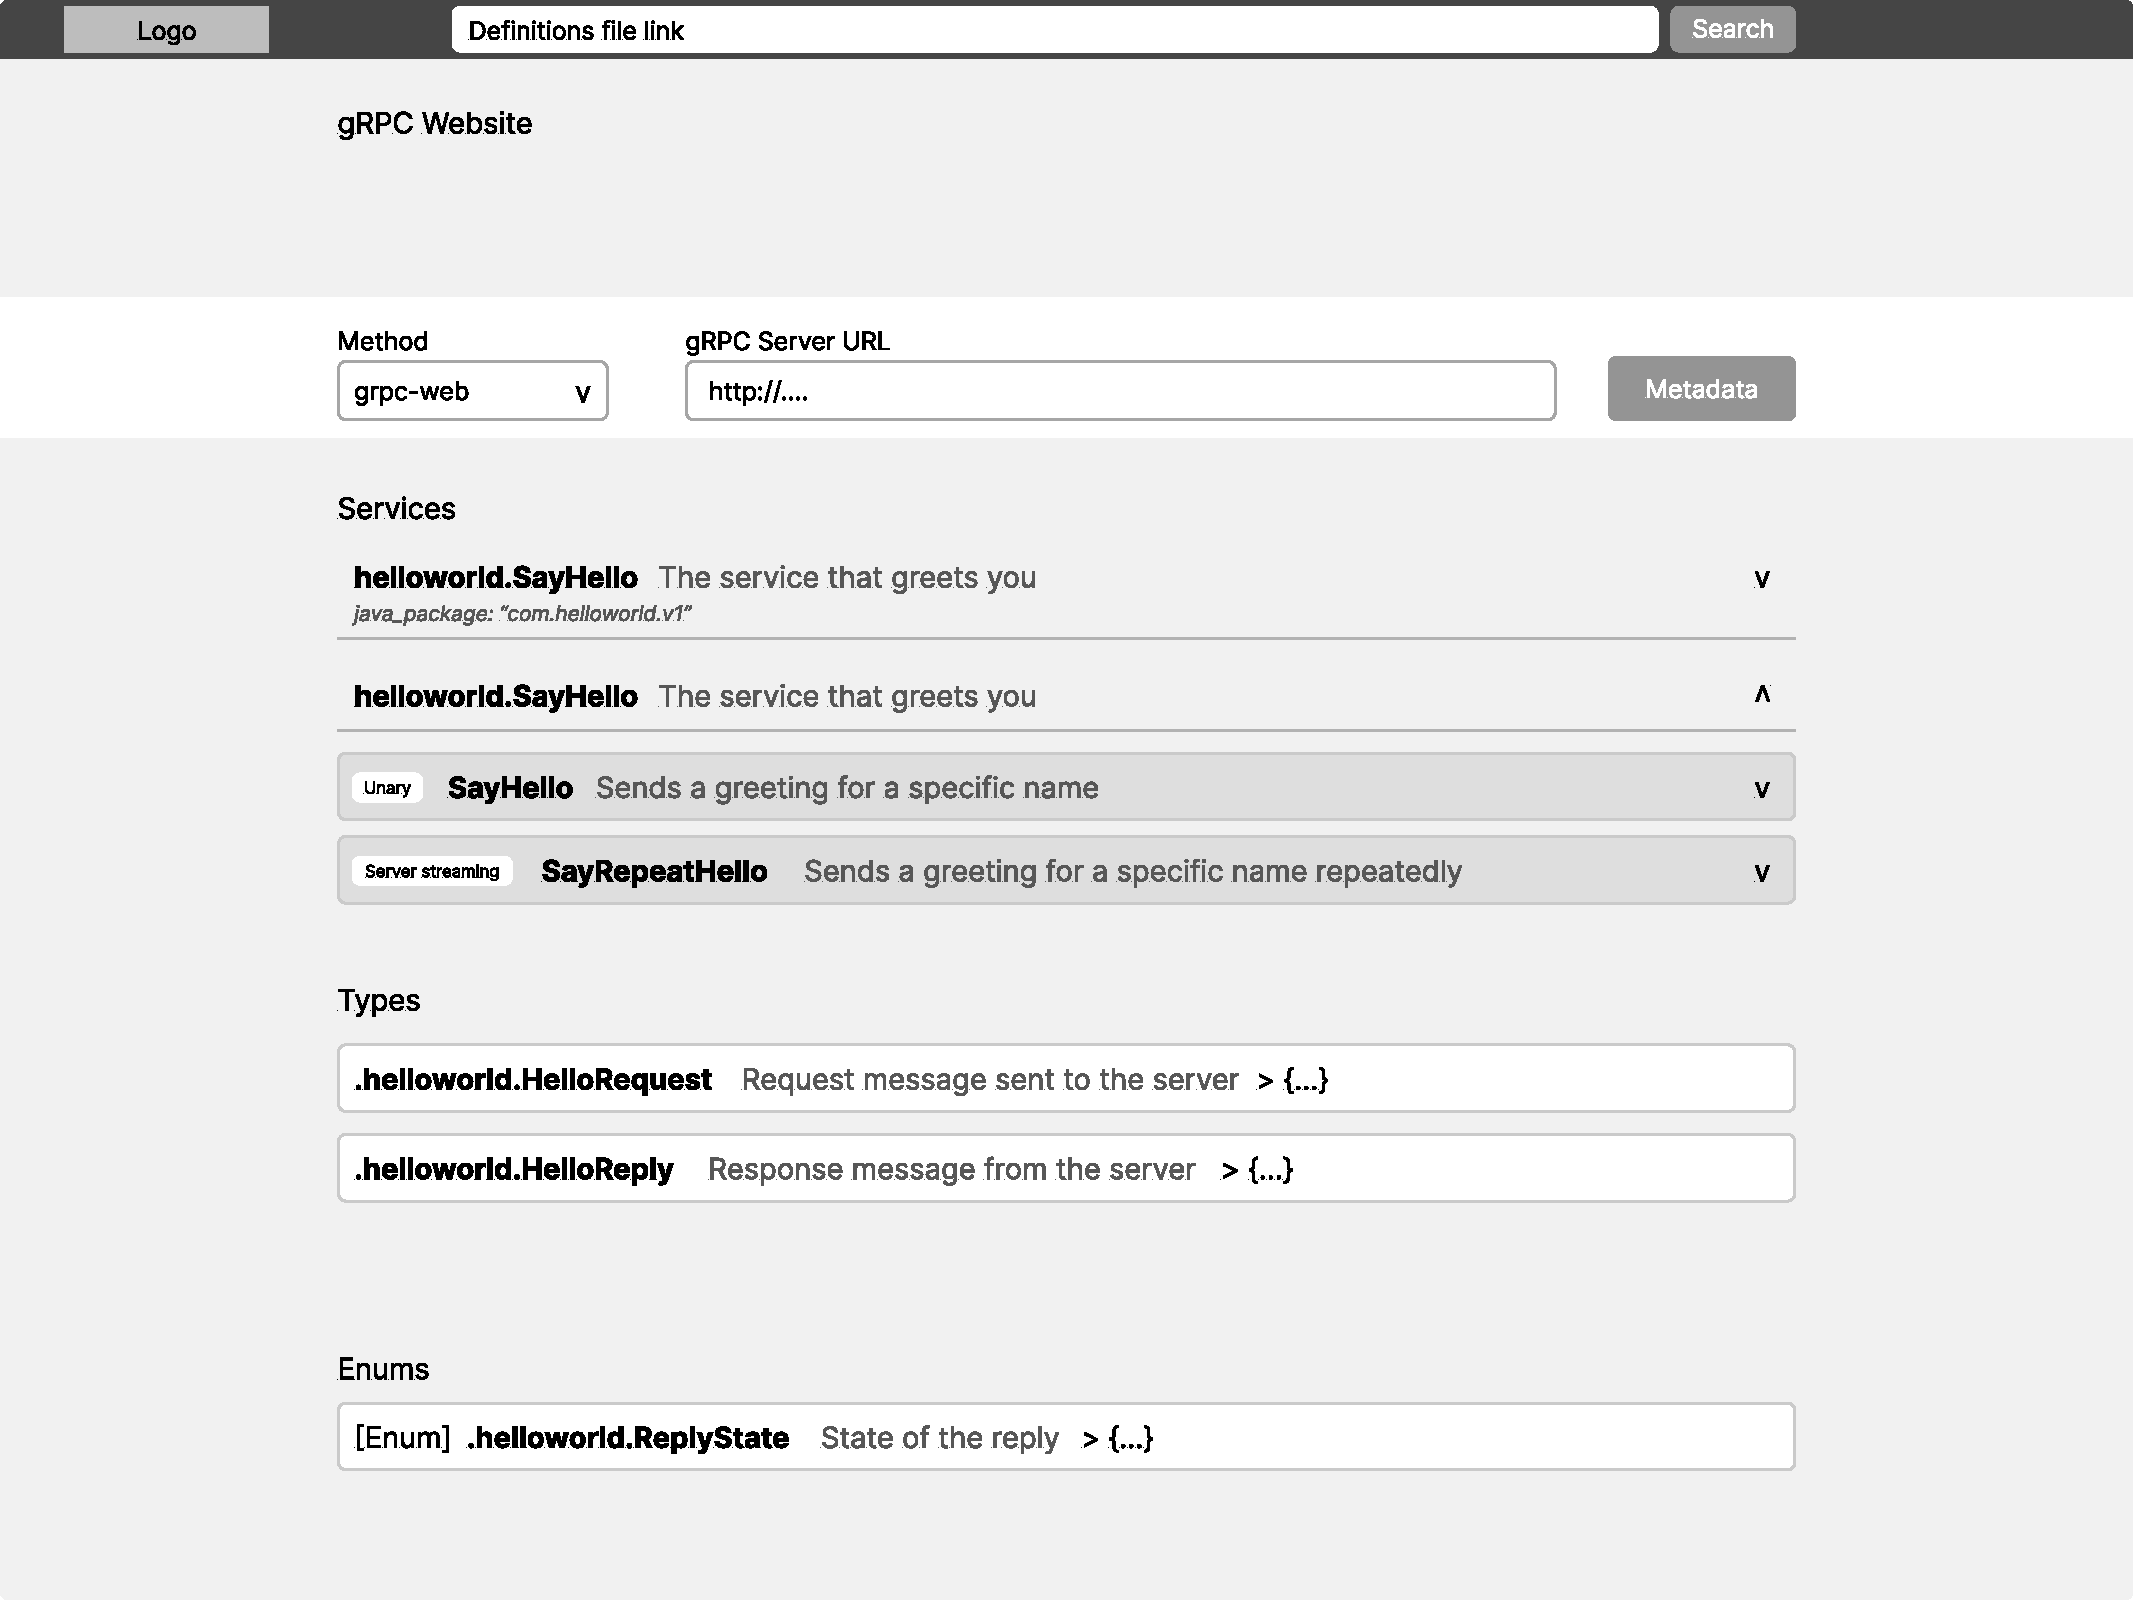
\includegraphics[width=1.0\textwidth]{images/design/wireframes/main-layout}
    \caption{Main Layout Wireframe}
    \label{fig:wireframe-main-layout}
\end{figure}

\subsubsection{Method Wireframe}
% Section: Method and its detail with forms, JSON, etc
The method wireframe is shown in the figure~\ref{fig:wireframe-method}.
It contains the method name, type, full documentation comment, and options.
Then, it is divided into two sections.
The first one contains the request data, and the second one contains the response data.

The request data section contains a table with all top-level fields and their respective names, types, and comments.
All fields are empty by default because all fields in the gRPC request are optional by design.
The only pre-filled fields are message types because the structures can be complex, and I assume they will be filled with at least some data.
If not, they can be cleared by the user, which I consider to be easier than creating the structure from scratch.
Additional options are shown for these fields, too.
These options allow the user to preview an example input and the target message type model.
The input of the message type is done using a JSON format, which is validated on the fly.
The form itself is generated only for the top-level fields, and the example input is done only for one level deeper.
This is an intentional design decision because the depth of nested message types can be infinite, but the user input always starts with the top-level one.
Therefore, any nested message type is treated as being part of the top-level message type.
This should allow quick input for common use cases, such as one string or number of inputs, but also be able to define complex structures using the JSON format for message types.
For fields using oneof, repeated, or map, respective implementations, such as an array, are shown.

Before the request execution, all fields are validated, and the user is informed about any errors.
Message type errors that do not conform to the message type structure are shown, too.
This should allow the user to correct the errors and execute the request again.

The responses section contains content type selection, which is used mainly for the gRPC-Web and sets the content type of the communication, and four subsections:
\begin{itemize}
    \item request JSON,
    \item request server,
    \item server responses,
    \item responses.
\end{itemize}

The content type selection place is based on the Swagger UI content type selection, hence part of the responses section.
The request JSON section contains the request data in JSON format with metadata, which is sent to the server.
This is useful for debugging purposes, as the user can see what is sent to the server in case the UI is not clear enough.
The request server section contains the information about the request server to remind the user that this server is requested because its URL is set in the global settings at the top of the page.
The server responses section contains information about the server responses, such as headers, status codes (if an error occurred), messages, and trailers.
The messages are dynamically added in this section in the case of server streaming-type requests.
The responses section contains an example response from the server in the case of success with the example message type.
The message type is expandable and behaves the same as I will describe in the following message type detail section.


\begin{figure}[hbt!]
    \centering
    \captionsetup{justification=centering}
    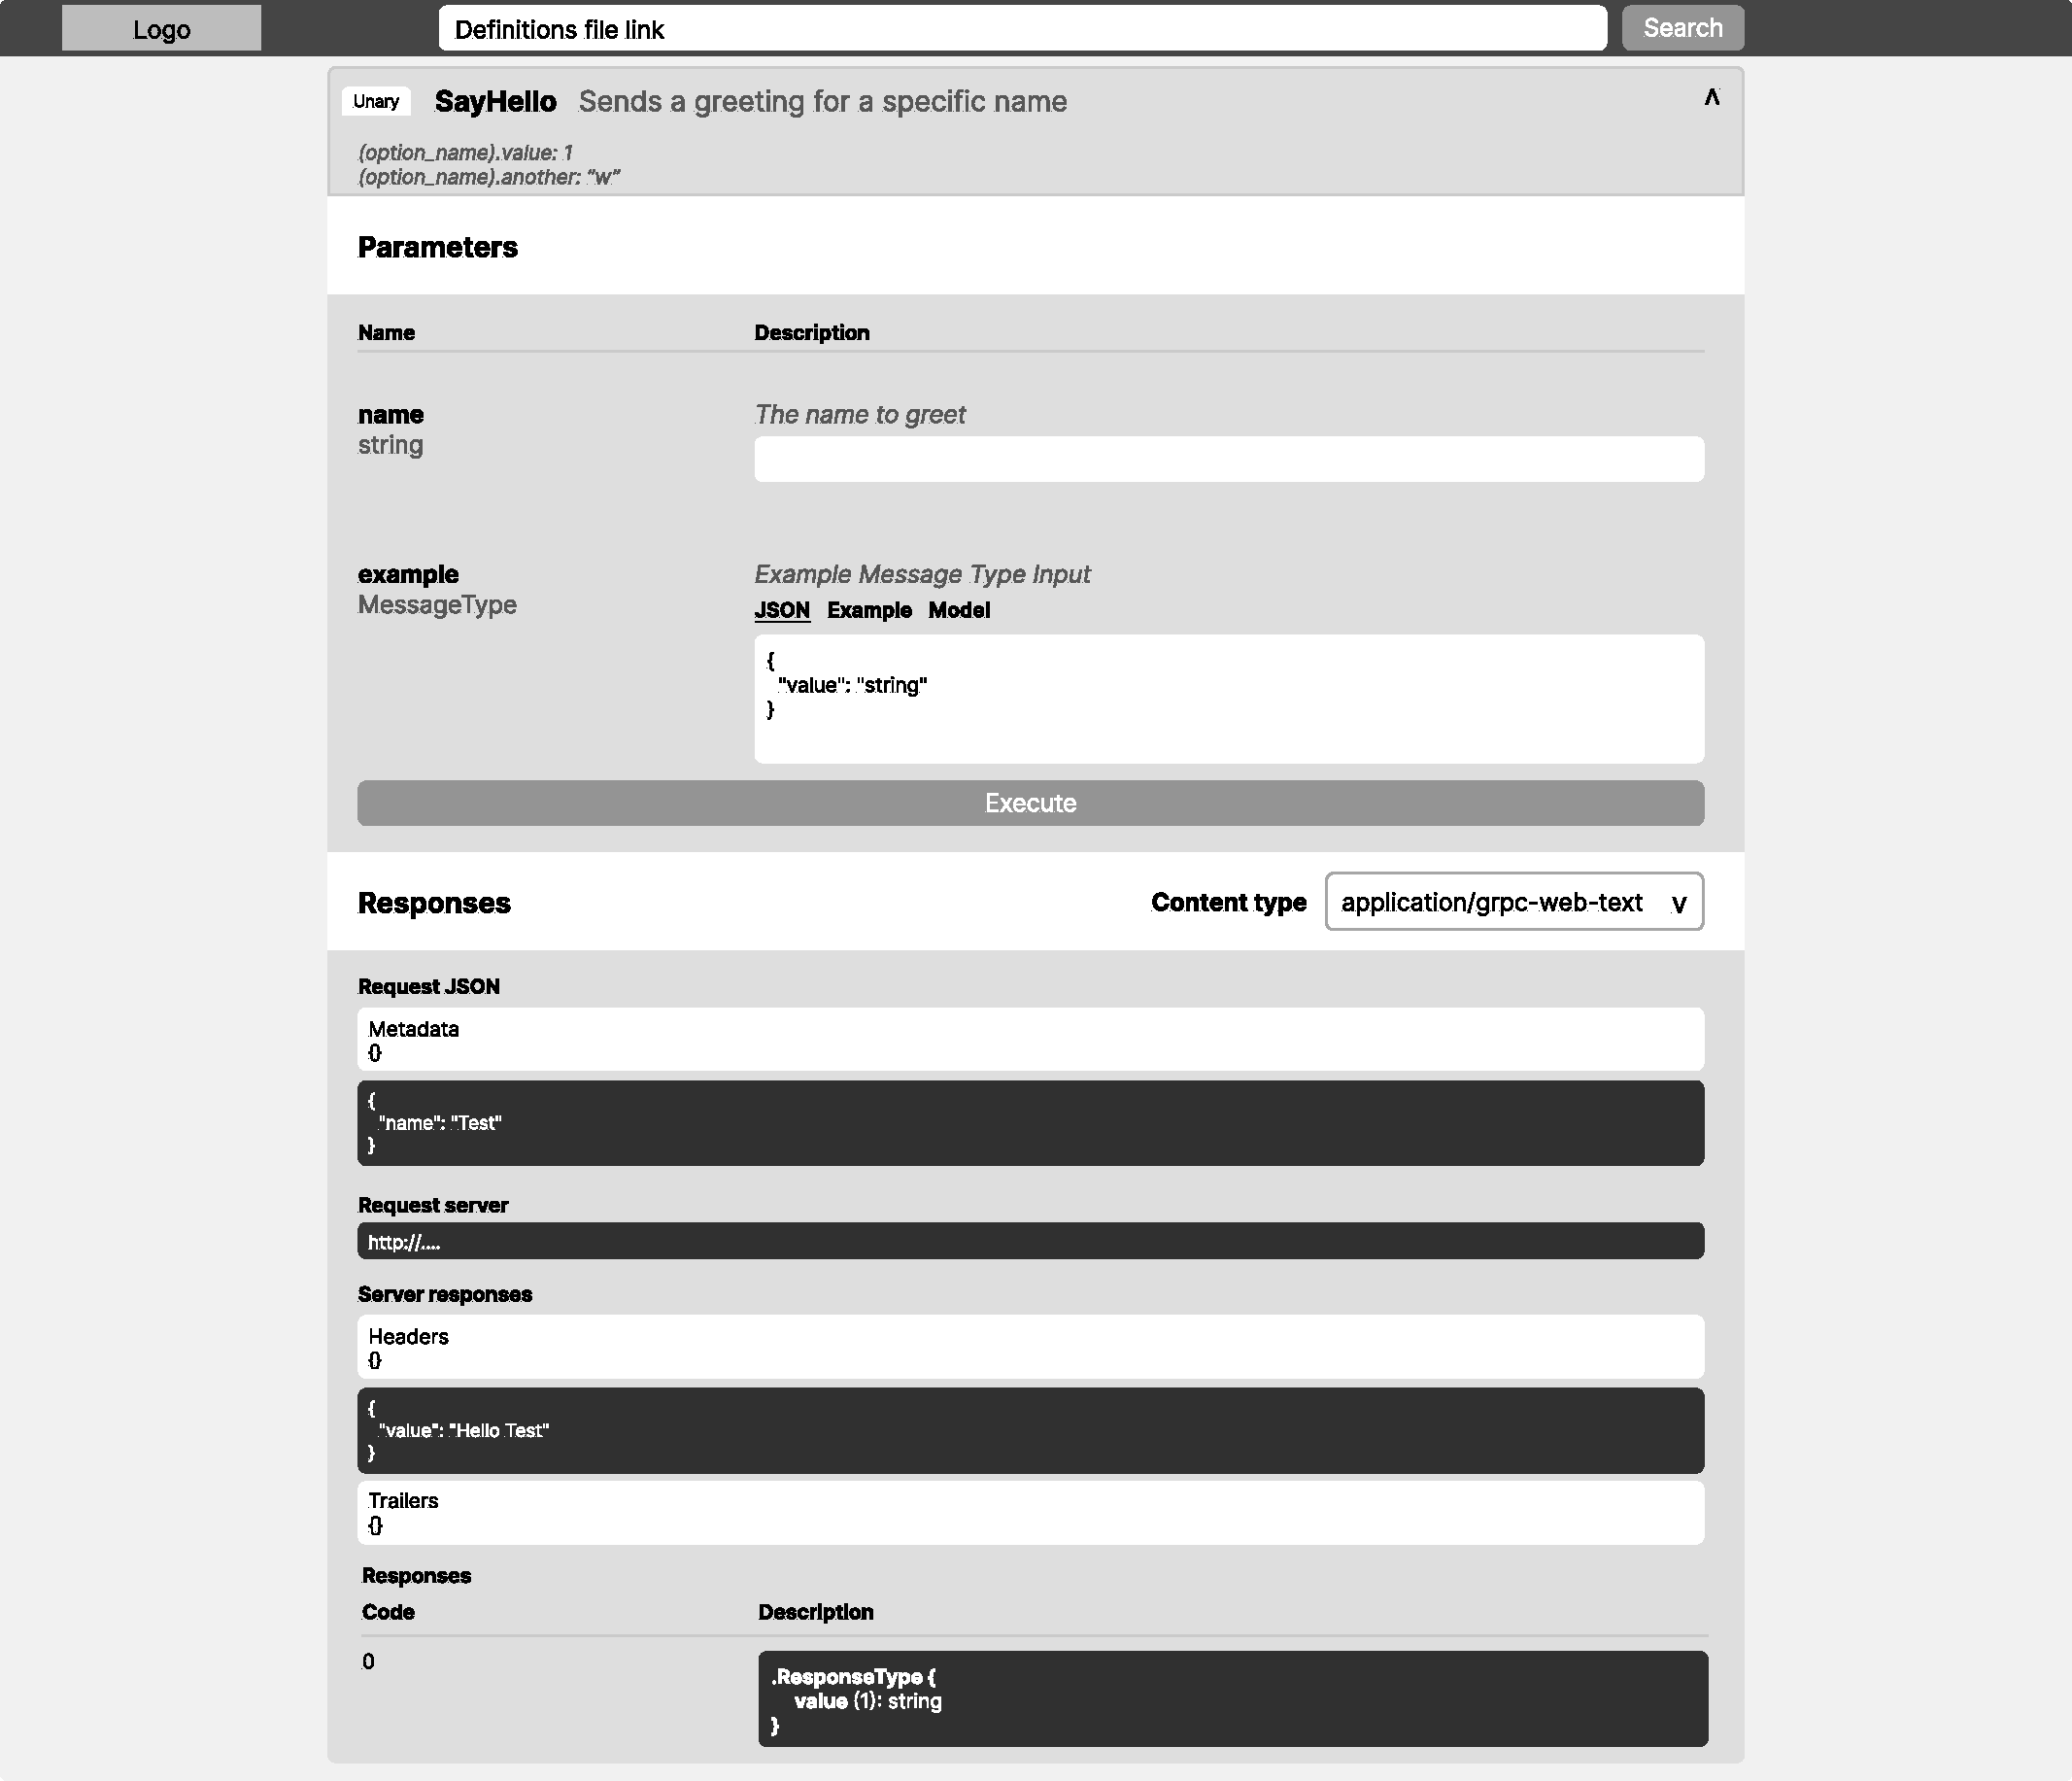
\includegraphics[width=1.0\textwidth]{images/design/wireframes/method}
    \caption{Method Wireframe}
    \label{fig:wireframe-method}
\end{figure}

\subsubsection{Type and Enum Wireframe}
The method wireframe is shown in the figure~\ref{fig:wireframe-type} and the enum wireframe in the figure~\ref{fig:wireframe-enum}.
Both message types and enums contain the full package path with a name and a documentation comment and can be expanded to show more information.
They also include options like \textit{allow\_alias} for enums.

For the message types, all fields are shown with their names, documentation comments, unique identifiers, and types.
Also, fields that are part of oneof, repeated, or map are shown in their respective manner.
If the field type is a message type, it is expandable as well, and it shows the same information as the message type itself.
Recursive message types allow infinite expansion.

\begin{figure}[hbt!]
    \centering
    \captionsetup{justification=centering}
    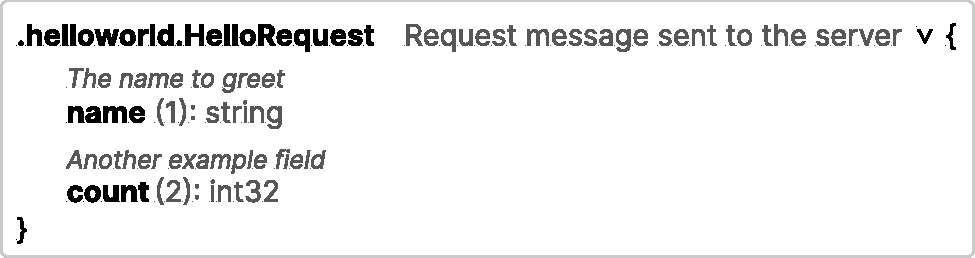
\includegraphics[width=0.8\textwidth]{images/design/wireframes/type}
    \caption{Type Wireframe}
    \label{fig:wireframe-type}
\end{figure}


For the enums, all keys are shown with their values and value options.
The value options can be used, for example, to mark the key as deprecated or define custom properties.

\begin{figure}[hbt!]
    \centering
    \captionsetup{justification=centering}
    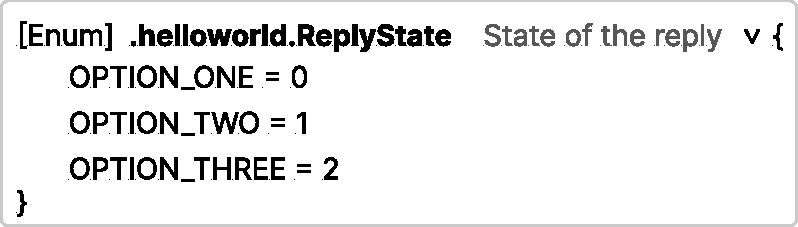
\includegraphics[width=0.8\textwidth]{images/design/wireframes/enum}
    \caption{Enum Wireframe}
    \label{fig:wireframe-enum}
\end{figure}

Both message types and enum types work the same when used in the method requests and response examples, and they are expandable on demand with the same design.
The support for well-known types is achieved by traversing all imported dependencies and showing their definitions.
They are shown in the same way as the user-defined types.


\section{Fulfillment of Requirements}
I have gone through all the requirements and added a description of how the website design fulfills them.
It is shown in the table~\ref{tab:requirements-fulfillment}.

Based on the table, the website generator design fulfills all the requirements defined in the analysis.

\begin{landscape}
    \begin{table}[!ht]
        \centering
        \resizebox{\columnwidth}{!}{%
            \renewcommand{\arraystretch}{2}
            \begin{tabular}{|p{0.3\linewidth}|l|l|l|l|l|l|l|l|l|l|l|l|l|l|l|l|l|l|l|l|l|l|l|l|}
                \hline
                \textbf{}                                                                                                      & \textbf{F1} & \textbf{F2} & \textbf{F3} & \textbf{F4} & \textbf{F5} & \textbf{F6} & \textbf{F7} & \textbf{F8} & \textbf{F9} & \textbf{F10} & \textbf{F11} & \textbf{F12} & \textbf{F13} & \textbf{F14} & \textbf{F15} & \textbf{F16} & \textbf{F17} & \textbf{F18} & \textbf{F19} & \textbf{F20} & \textbf{F21} & \textbf{N1} & \textbf{N2} & \textbf{N3} \\ \hline
                \textbf{Main webpage design}                                                                                   & x           & x           & x           & ~           & ~           & ~           & ~           & ~           & ~           & ~            & ~            & ~            & ~            & ~            & ~            & ~            & ~            & ~            & ~            & ~            & ~            & ~           & ~           & ~           \\ \hline
                \textbf{Showing comments for the services, methods, message types, fields, and enums} & ~ & ~ & ~ & x & x & ~ & ~ & ~ & ~ & ~ & ~ & ~ & ~ & ~ & ~ & ~ & ~ & ~ & ~ & ~ & ~ & ~ & ~ & ~ \\ \hline
                \textbf{Execution of methods using direct gRPC-Web implementation}                                             & ~           & ~           & ~           & ~           & ~           & x           & x & ~ & ~ & ~ & ~ & ~ & ~ & ~ & ~ & ~ & ~ & ~ & ~ & ~ & ~ & ~ & ~ & ~ \\ \hline
                \textbf{Method design with inputs for all fields}                                                              & ~           & ~           & ~           & ~           & ~           & ~           & ~           & x           & ~           & ~            & ~            & ~            & ~            & ~            & ~            & ~ & ~ & ~ & ~ & ~ & ~ & ~ & ~ & ~ \\ \hline
                \textbf{Form validation}                                                                                       & ~           & ~           & ~           & ~           & ~           & ~           & ~           & ~           & x           & ~            & ~            & ~            & ~            & ~            & ~            & ~            & ~            & ~            & ~            & ~            & ~            & ~           & ~           & ~           \\ \hline
                \textbf{Global metadata settings, with the ability to set the authorization token} & ~ & ~ & ~ & ~ & ~ & ~ & ~ & ~ & ~ & x & ~ & ~ & ~ & ~ & ~ & ~ & ~ & ~ & ~ & x & ~ & ~ & ~ & ~ \\ \hline
                \textbf{Showing the response headers, messages as they come, and trailers}                                     & ~           & ~           & ~ & ~ & ~ & ~ & ~ & ~ & ~ & ~ & x & x & ~ & ~ & ~ & ~ & ~ & ~ & ~ & ~ & ~ & ~ & ~ & ~ \\ \hline
                \textbf{Supporting oneof, map, repeated, and nested message types in the method input and in the message type} & ~ & ~ & ~ & ~ & ~ & ~ & ~ & ~ & ~ & ~ & ~ & ~ & x & x & x & x & ~ & ~ & ~ & ~ & ~ & ~ & ~ & ~ \\ \hline
                \textbf{Supporting all imported types, including well-known types, and showing them in the types section} & ~ & ~ & ~ & ~ & ~ & ~ & ~ & ~ & ~ & ~ & ~ & ~ & ~ & ~ & ~ & ~ & x & ~ & ~ & ~ & ~ & ~ & ~ & ~ \\ \hline
                \textbf{Generator for the proto files}                                                                         & ~           & ~           & ~           & ~           & ~           & ~           & ~           & ~           & ~           & ~            & ~            & ~            & ~            & ~            & ~            & ~            & ~            & x            & ~            & ~            & ~ & ~ & ~ & ~ \\ \hline
                \textbf{gRPC reflection generator, combined with grpcurl}                                                      & ~           & ~           & ~           & ~           & ~           & ~           & ~           & ~           & ~           & ~            & ~            & ~ & ~ & ~ & ~ & ~ & ~ & ~ & x & ~ & ~ & ~ & ~ & ~ \\ \hline
                \textbf{Showing options for services, methods, message types, and enum values}                                 & ~ & ~ & ~ & ~ & ~ & ~ & ~ & ~ & ~ & ~ & ~ & ~ & ~ & ~ & ~ & ~ & ~ & ~ & ~ & ~ & x & ~ & ~ & ~ \\ \hline
                \textbf{Website is static and all content is generated on the fly}                                             & ~           & ~           & ~           & ~           & ~           & ~           & ~ & ~ & ~ & ~ & ~ & ~ & ~ & ~ & ~ & ~ & ~ & ~ & ~ & ~ & ~ & x & ~ & ~ \\ \hline
                \textbf{UI is inspired by the Swagger UI design, and it is adjusted to the gRPC specifics} & ~ & ~ & ~ & ~ & ~ & ~ & ~ & ~ & ~ & ~ & ~ & ~ & ~ & ~ & ~ & ~ & ~ & ~ & ~ & ~ & ~ & ~ & x & ~ \\ \hline
                \textbf{Message request input is in a combination of form and JSON format}                                     & ~           & ~           & ~ & ~ & ~ & ~ & ~ & ~ & ~ & ~ & ~ & ~ & ~ & ~ & ~ & ~ & ~ & ~ & ~ & ~ & ~ & ~ & ~ & x \\ \hline
            \end{tabular}
        }
        \caption{Fulfillment of requirements}
        \label{tab:requirements-fulfillment}
    \end{table}
\end{landscape}